\section{Test 1: Escenario simple, unico punto de acceso}
La red más sencilla es por defecto la red de un punto de acceso y dos estaciones wireless. El punto de acceso está conectado directamente al controlador, y las estaciones wireless serán los host. La idea de este test es comprobar que hay fluctuación de tráfico de control OpenFlow en el punto de acceso y además hay tráfico de usuario en la interfaz de wlan.
\subsection{Capturando tráfico de control wireless en Mininet-Wifi}
\begin{itemize}
    \item Lanzamos Wireshark para analizar tráfico: \textbf{wireshark \&}
    \item Lanzamos Mininet-Wifi con el siguiente comando, además por defecto cargará la topología por defecto(Valga la redundancia): \textbf{sudo mn -wifi}
    \item Lo siguiente, es activar la interfaz hwsim0. Pero, ¿Qué es la interfaz hwsim0? La interfaz hwsim0 es una interfaz software creada por Mininet-Wifi que copia todo el trafico wireless  dirigido a todas las interfaces wireless virtuales de la topología a emular. Según la documentación seguida es la forma más sencilla de monitorizar los mensajes wireless en Mininet-Wifi. Desde la Mininet-Wifi CLI: \textbf{sh ifconfig hwsim0 up} 
    \begin{itemize}
        \item El comando \textbf{sh} en la CLI de Mininet tiene la funcionalidad de ejecutar un comando fuera de la Interfaz de Mininet-Wifi.
    \end{itemize}
    
    \item Una vez levantada la interfaz podemos poner Wireshark a escuchar en la interfaz.
    
    \item Hacemos Ping desde la estación sta1, a la estación sta2: \textbf{sta1 ping sta2}
    
    \item Comprobamos que hay tráfico escuchando en la interfaz:
    
    
\end{itemize}
\newpage
\begin{figure}[!htb]
  \centering
    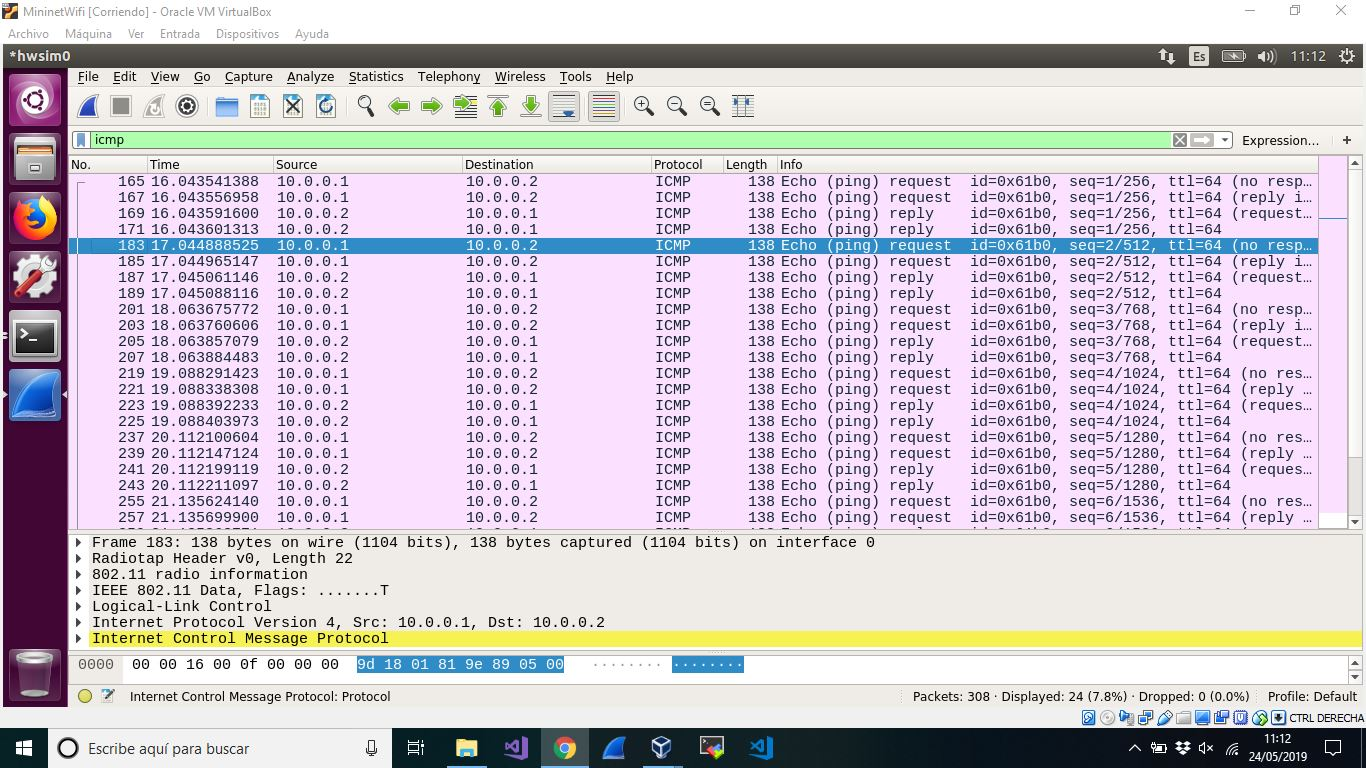
\includegraphics[width=\linewidth]{./img/test/5.JPG}
    \caption{Comprobación que hay trafico a través de la interfaz.}
  \label{fig:yo}
\end{figure}

Como podeos ver el punto de acceso tiene una interfaz asociada llamada ap1-wlan1. Por defecto, las estaciones wireless asociadas con el punto de acceso se conectan en modo "\textbf{infrastructure} " esto significa que el tráfico wireless entre dos estaciones asociadas al punto de acceso debe pasar siempre a través de este. Sabiendo que los puntos de acceso funcionan de forma similar a los switch en Mininet, esperaríamos observar tráfico de control entre el punto de acceso y el controlador, cuando el punto de acceso,  observe tráfico para el cual no se establecido una regla (No pertenece a un flujo para el cual haya asignada una acción en la tabla de flujos). 

\begin{figure}[!htb]
  \centering
    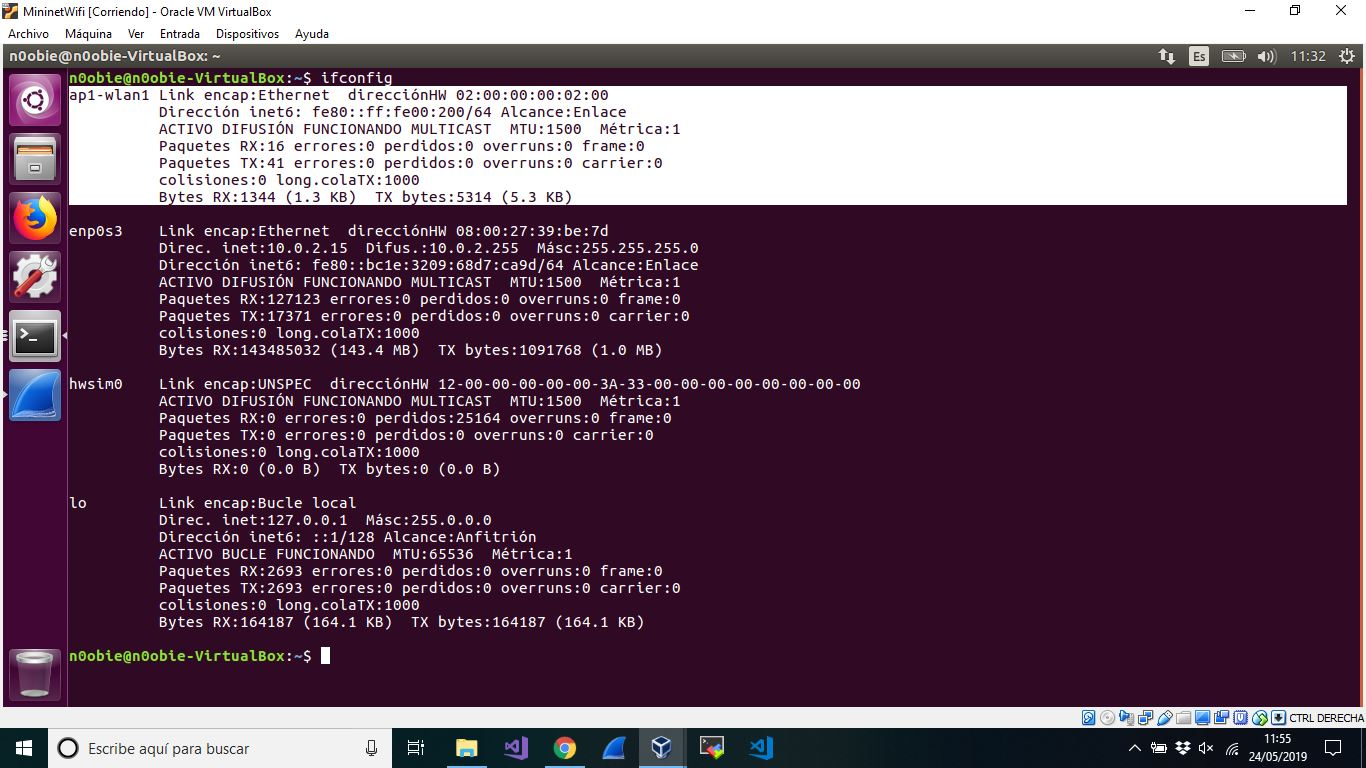
\includegraphics[width=0.9\linewidth]{./img/test/6.JPG}
    \caption{Interfaz ap1-wlan1 del Punto de acceso.}
  \label{fig:yo}
\end{figure}
\newpage
\subsection{Puntos de acceso Wireless y OpenFlow}
Si deseamos ver \textbf{paquetes OpenFlow}, debemos poner a escuchar Wireshark  en la interfaz de \textbf{loopback}. Podemos además utilizar el filtro: \textbf{OpenFlow\_1.0} para visualizarlo de una forma más clara. Dicho esto, ponemos a capturar Wireshark y repetimos el ping entre sta1 y sta2.
\begin{figure}[!htb]
  \centering
    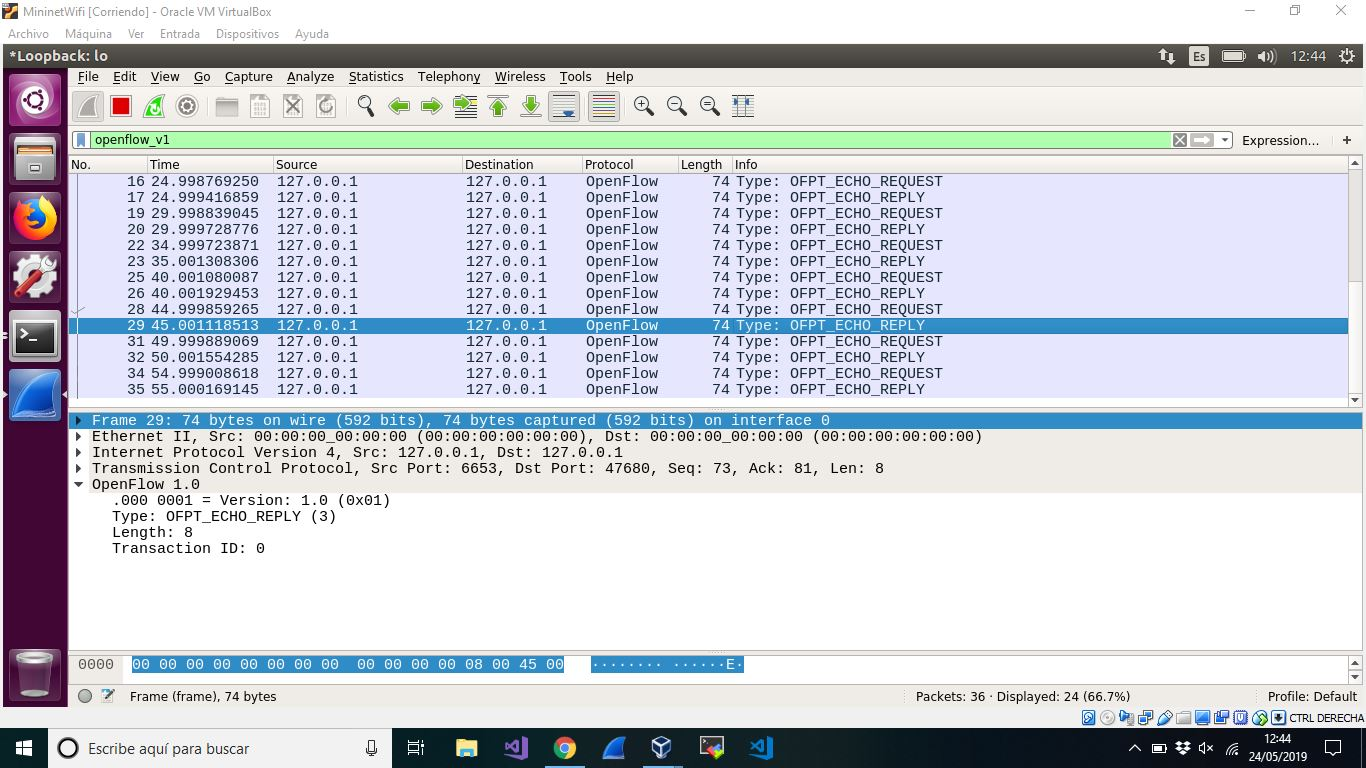
\includegraphics[width=\linewidth]{./img/test/7.JPG}
    \caption{Tráfico OpenFlow.}
  \label{fig:yo}
\end{figure}
\newline
Nota: 
\begin{itemize}
    \item Consultar comando dpctl: \url{http://ranosgrant.cocolog-nifty.com/openflow/dpctl.8.html}
    \item xID: Identificador de transacción, es aleatorio, identificador controlador - switch, va cambiando a lo largo del tiempo.  
    \item El estándar es OpenFlow 1.3, pero Mininet-Wifi funciona con OpenFlow 1.1
\end{itemize}

Como esperábamos el paquete ICMP debería ser redirigido al controlador para decidir que hacer con el paquete, al no tener un Flow con una regla establecida. De esta manera el controlador cuando  le llegue el paquete instanciará una serie de reglas en los switch para que el paquete ICMP sea encaminado de un host a otro. En cambio, encontramos que las dos estaciones son capaces de intercambiar paquetes inmediatamente sin redirigir el primer paquete al controlador. Solo una trama ARP , que es de tipo broadcast, es llevada hacia el controlador y es ignorada.\newline
\newline
Para comprobar si hubira algún flujo con una ccción instanciada en alguna de las estaciones bases hacemos:
\textbf{dpctl dump-flows}
\newline
\newline
Al hacer esto en esta altura del tutorial, vemos que no hay ninguna regla instanciada en la estación. ¿Pero, tiene esto sentido?¿Cómo se han comunicado las dos puntos de acceso?\newline
\newline
Según la guía, podemos apreciar que los switches con OpenFlow activado, van a rechazar las "Hairpin connections". Las cuales son flows que hacen que el tráfico, sea enviado por el mismo puerto que ha sido recibido.

\begin{itemize}
    \item \textbf{Hairpin connection}: Comunicación entre dos dispositivos host en el mismo dominio NAT utilizando sus puertos finales(Ya traducidos)
\end{itemize}
\newpage
\begin{figure}[!htb]
  \centering
    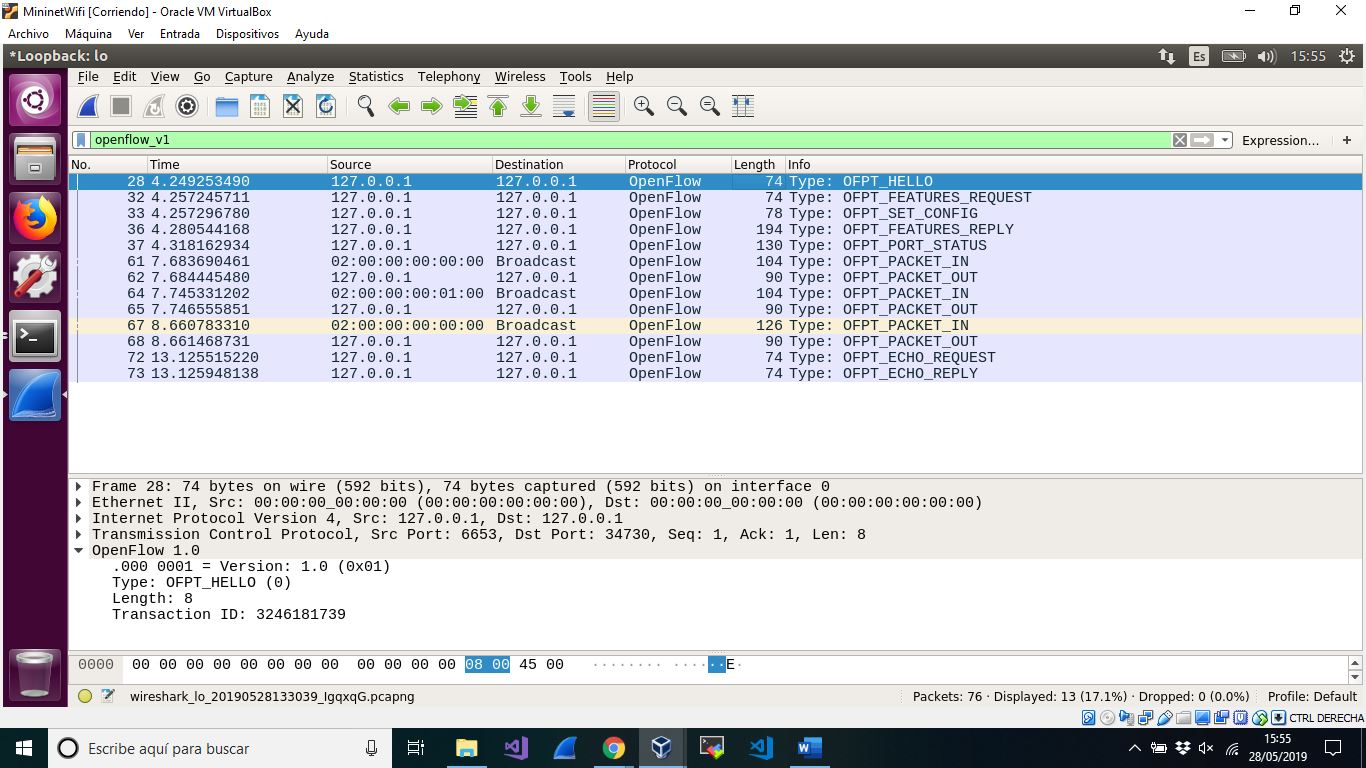
\includegraphics[width=\linewidth]{./img/test/8.JPG}
    \caption{No hay tráfico OpenFlow hacia el controlador.}
  \label{fig:yo}
\end{figure}
Un punto de acceso wireless, por diseño, recibe y manda paquetes en la misma interfaz. Las estaciones wifi conectadas al mismo punto de acceso requerirán a "Hairpin connection" para comunicarse entre ellas. El autor de la guía supone que Linux, maneja a la interfaz WLAN en cada punto de acceso como un enlace radio sta1-ap1-sta2 como si fuera un HUB, donde ap1-wlan0 proporciona la funcionalidad de "HUB"
para los datos que pasan entre sta1 y sta2.
ap1-wlan0 cambia los paquetes en el dominio inalámbrico y lo hará
no introduzca un paquete en la parte del "conmutador Ethernet" del punto de acceso ap1 a menos que deba cambiarse a
otra interfaz en ap1 que no sea ap1-wlan0.\newline
\newline
\begin{itemize}
    \item Podemos detener el ping con CTRL+C
    \item Podemos detener Mininet-Wifi vía comando \textbf{exit}
    \item Podemos limpiar los archivos residuales de Mininet-Wifi con:  \textbf{sudo mn -c}
\end{itemize}

\section{Test 2: Multiples puntos de acceso}
En este test vamos a crear una topología lineal con tres puntos de acceso, y tres estaciones wifi. Donde cada una está conectada a cada punto de acceso.\newline
\newline
Podemos crear la topología: \textbf{sudo mn --wifi --topo linear,3}
\newpage
\begin{figure}[!htb]
  \centering
    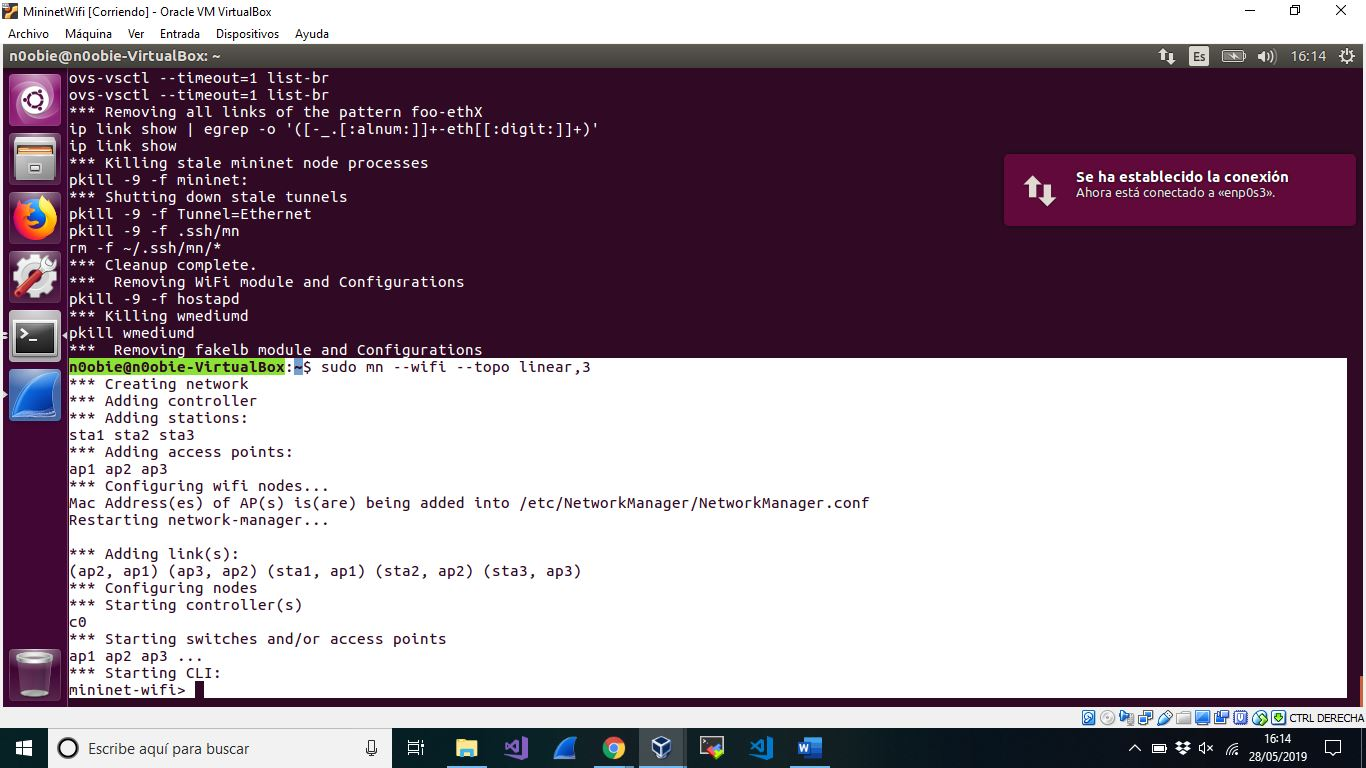
\includegraphics[width=\linewidth]{./img/test/9.JPG}
    \caption{Montar topología lineal en Mininet-Wifi.}
  \label{fig:yo}
\end{figure}
Además,  podemos  verificar la configuración de la topología haciendo uso de los comandos \textbf{net} y \textbf{dump}. Con el comando \textbf{net} podemos ver la conexión entre los nodos. Con el comando \textbf{dump} podemos ver la conexión entre los nodos y además información extra como el PID.\newline
\newline
Podemos contemplar que tenemos los tres puntos de acceso conectados juntos entre ellos uno a uno de una manera lineal mediante enlaces de Ethernet. Pero, no vemos ningún tipo de información sobre las estaciones Wifi, en lo relativo a que punto de acceso están conectadas. Esto se debe a que esa conexión se lleva a cabo mediante un enlace te tipo radio. Para poder consultar esta información tendremos que hacer uso del comando \textbf{iw} (Interface Wireless) en cada estación Wifi para poder contemplar a que punto de acceso está conectada. \newline
\newline
Para poder verificar que puntos de acceso son alcanzables por una estación Wifi usaremos \textbf{staX iw dev staX-wlan0 scan}. Para afinar la busqueda podemos hacer un grep del ssid para quitarnos información extra.\newline
\newline
\begin{center}
    \textbf{sta1 iw dev sta1-wlan0 scan | grep ssid}
\end{center}
\begin{figure}[!htb]
  \centering
    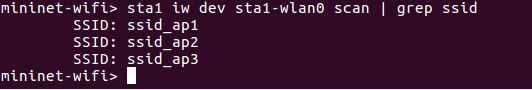
\includegraphics[width=0.5\linewidth]{./img/test/10.JPG}
    \caption{Comprobar que puntos de accesos son alcanzables en Mininet-Wifi.}
  \label{fig:yo}
\end{figure}
Para comprobar a que punto de acceso está conectado en un momento dado una estación Wifi podemos hacerlo mediante el comando \textbf{iw link}. Por ejemplo: \textbf{sta1 iw dev sta1-wlan0 link
}
\newpage
\begin{figure}[!htb]
  \centering
    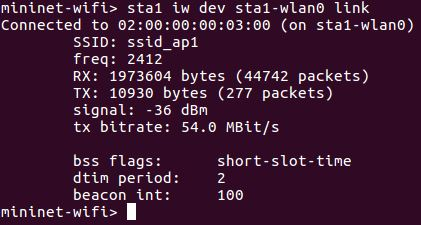
\includegraphics[width=0.5\linewidth]{./img/test/11.JPG}
    \caption{Comprobar el punto de acceso actual en Mininet-Wifi.}
  \label{fig:yo}
\end{figure}
Con este comando  podemos apreciar distintas estadísticas como pueden ser la potencia de señal recibida, la cantidad de bytes transmitidos y recibidos, el régimen binario de transmisión, SSID, y la frecuencia expresada en MHz, en este caso se trata del canal 1 Wifi. Debemos recordar que el espectro Wifi se extiende desde 2402 MHz hasta los 2494 Mhz (La banda de los 2.4GHz).\newline
\newline
En este caso cada estación Wifi está conectad a un punto de acceso según se pudo ver con los anteriores comandos de \textbf{net} y \textbf{dump}. Se puede hacer uso del comando \textbf{iw} para conmutar de un punto de acceso por otro. \newline
\newline
Nota de la guia: \textit{Los comandos iw pueden usarse en escenarios estáticos como este, pero no deben usarse cuando
Mininet-WiFi asigna automáticamente asociaciones en escenarios de movilidad más realistas. Discutiremos
cómo Mininet-WiFi maneja la movilidad real y cómo usar los comandos iw con Mininet-WiFi más adelante
esta publicación}.
\subsection{Asociaciones con los puntos de acceso}
En este caso vamos a comprobar como podemos cambiar la conexión existente entre la estación Wifi 1 (sta1) con el punto de acceso 1 (ap1). En este caso vamos a conectar la estación Wifi 1 (sta1) con el punto de acceso 2 (ap2). Debemos recordar los SSID de cada punto de acceso (ssid\_apX).\newline
\newline
\begin{center}
\begin{itemize}
    \item  Para desconectarnos del actual punto de acceso:  \textbf{sta1 iw dev sta1-wlan0 disconnect}
    \item Para conectarnos a ap2: \textbf{sta1 iw dev sta1-wlan0 connect ssid\_ap2}
\end{itemize}
\end{center}
Podemos verificar el funcionamiento de este comando usando el comando iw link que ya se explico anteriormente.
\begin{figure}[!htb]
  \centering
    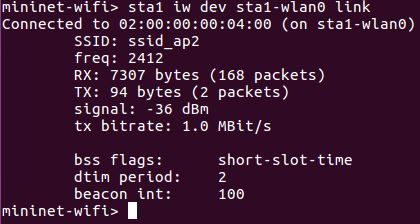
\includegraphics[width=0.5\linewidth]{./img/test/12.JPG}
    \caption{\textit{Handover} completado en Mininet-Wifi.}
  \label{fig:yo}
\end{figure}
Hemos podido comprobar como se puede hacer un simple \textit{Handover} entre dos puntos de acceso.
\newpage
Ahora vamos a estudiar como gestiona el controlador OVSAP de Mininet-Wifi el Handover entre dos células Wifi. Para llevar a cabo este experimento vamos hacer ping desde sta3 hacia sta1. Entraremos en la terminal de sta3 con el comando \textbf{xterm}. Para hacer ping debemos saber las distintas IPs de las distintas estaciones Wifi, podemos consultarlas con el comando \textbf{dump}.
\begin{figure}[!htb]
  \centering
    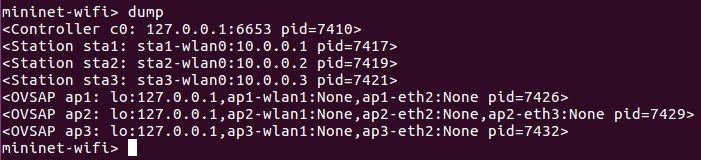
\includegraphics[width=\linewidth]{./img/test/13.JPG}
    \caption{Consultar IPs en Mininet-Wifi.}
  \label{fig:yo}
\end{figure}
\begin{figure}[!htb]
  \centering
    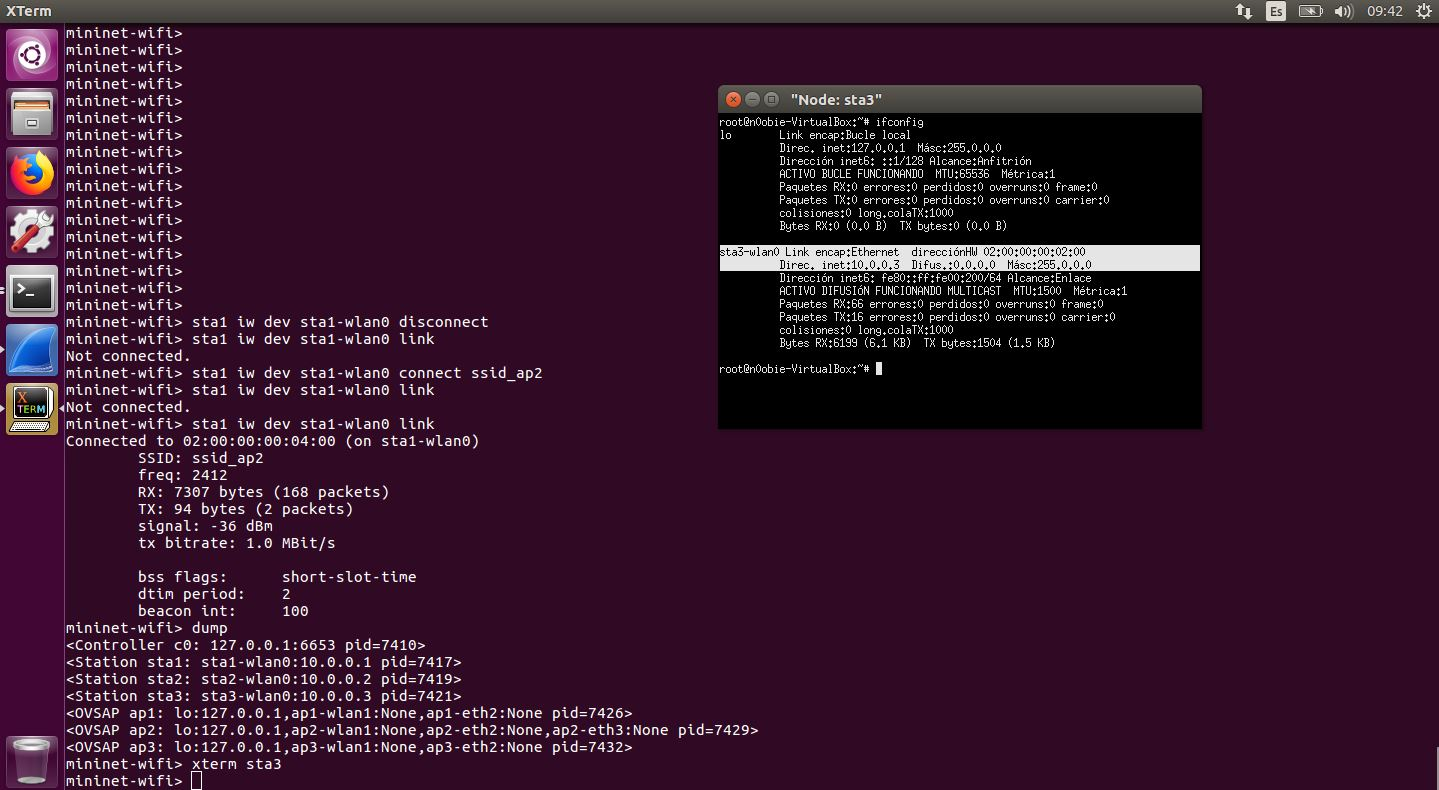
\includegraphics[width=\linewidth]{./img/test/14.JPG}
    \caption{Entrar en la consola de \textit{Sta3}.}
  \label{fig:yo}
\end{figure}
\newline
Vamos hacer ping desde sta3 a sta1 (\textbf{Ip: 10.0.0.1}). Ahora desde que estos paquetes serán reenviados por los puntos de acceso asociados, en un puerto distinto al puerto
en el que se recibieron los paquetes, los puntos de acceso funcionarán normalmente en cuanto a OpenFlow ser refiere. Cada punto de acceso va a reenviar el primer ping que le llegue en dirección al controlador. El controlador va a instanciar en las tablas de flows de cada punto de acceso las reglas correspondientes para que se pueda instanciar una conexión entre sta1 y sta3. \newline

\subsection{Flows OpenFlow en un escenario de Handover}
Podemos comprobar el intercambio de paquetes OpenFlow escuchando la interfaz de loopback.
\newpage
\begin{figure}[!htb]
  \centering
    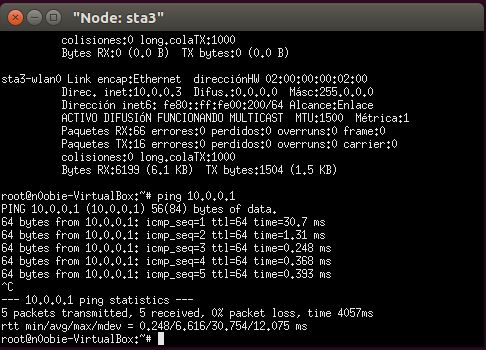
\includegraphics[width=0.8\linewidth]{./img/test/15.JPG}
    \caption{Ping desde \textit{Sta3} a \textit{Sta1}.}
  \label{fig:yo}
\end{figure}
\begin{figure}[!htb]
  \centering
    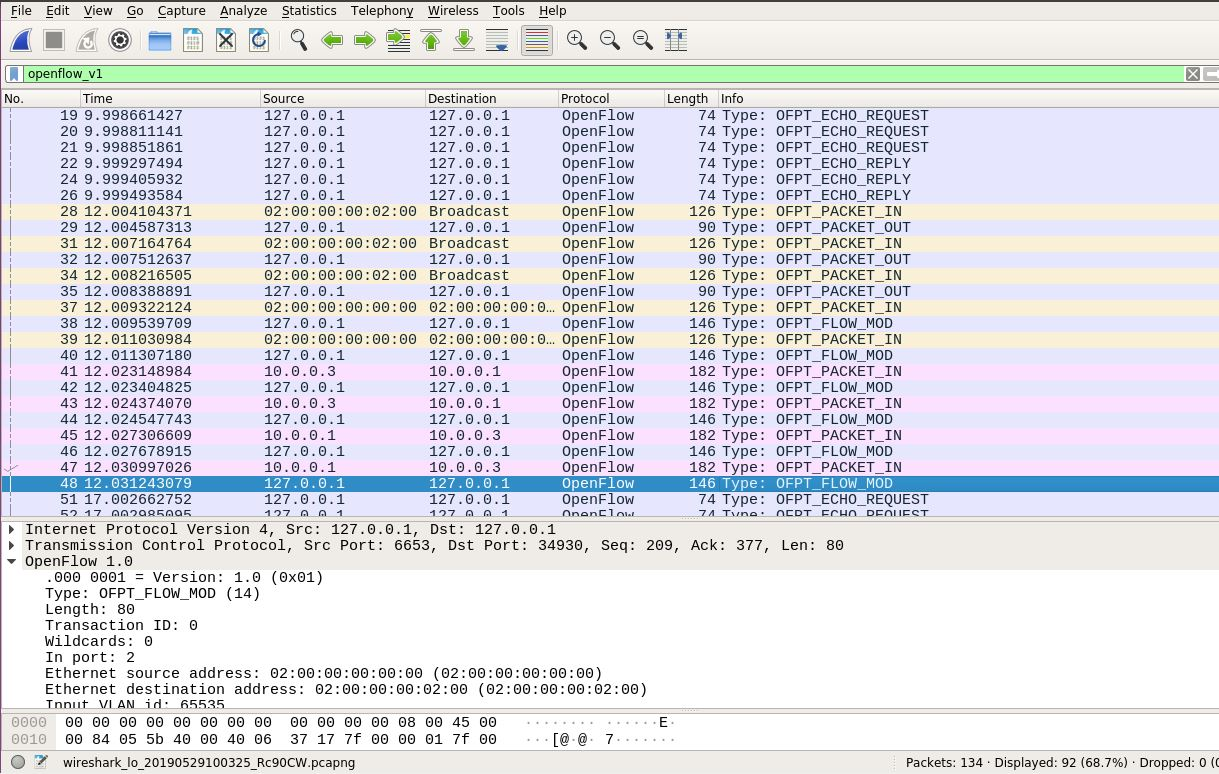
\includegraphics[width=\linewidth]{./img/test/16.JPG}
    \caption{Captura de Wireshark del ping.}
  \label{fig:yo}
\end{figure}
\newpage
Podemos apreciar como el punto de acceso ap3 empieza mandando el paquete de ARP request para que Sta3 sepa la \textit{MAC} de Sta1 hacia arriba para que decida que debe hacer con el controlador. El controlador hace un PACKET\_OUT. Para el ARP reply el controlador hace un PACKET\_IN. Una vez que Sta3 sabe sabe la dirección \textit{MAC} del destino se dispone a enviar el ping. El controlador instanciará un flow\_mod por cada punto de acceso, y otro para el ECHO reply del ping.

\begin{figure}[!htb]
  \centering
    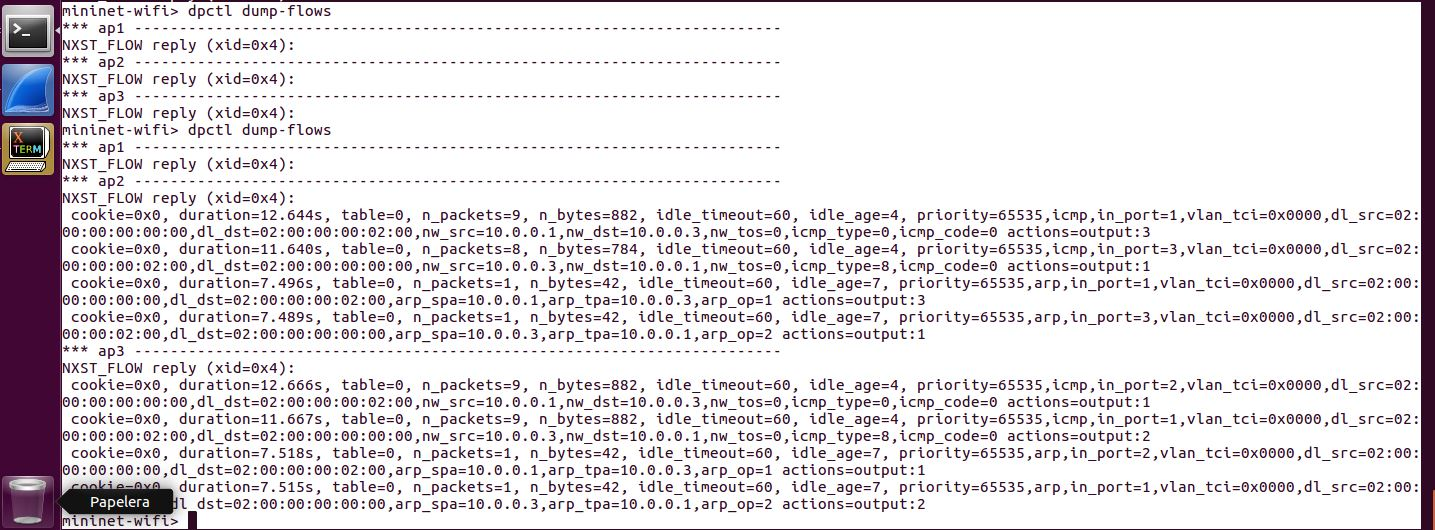
\includegraphics[width=\linewidth]{./img/test/17.JPG}
    \caption{Flow tables de los distintos puntos de acceso.}
  \label{fig:yo}
\end{figure}
\newline
Como se puede apreciar en la figura, al principio de la comprobación de las tablas de cada punto de acceso estaban vacias. Esto es ya que estas entradas en la tabla tienen un tiempo de vida, agotado se eliminan de la tabla. Por lo que al repetir el ping se vuelve a repetir el proceso de instanciar los Flow\_Mod en cada tabla de cada punto de acceso para poder llevarse así a cabo el ping. \newline
\newline

Pero resulta curioso el hecho de que en le punto de acceso 1 (ap1) no haya ninguna entrada en su tabla de Flows. Esto es ya que este punto de acceso no interviene ya que anteriormente hicimos un Handover de Sta1, entre ap1 y el ap2. Podemos comprobar que si volvemos a enlazar Sta1 con ap1, ap1 deberá tener también las entradas suficientes en su Flow table para poder llevar a cabo la conexión entre Sta1 y Sta3. 
\begin{itemize}
    \item \textbf{sta1 iw dev sta1-wlan0 disconnect} 
    \item \textbf{sta1 iw dev sta1-wlan0 connect ssid\_ap1}
\end{itemize}
\begin{figure}[!htb]
  \centering
    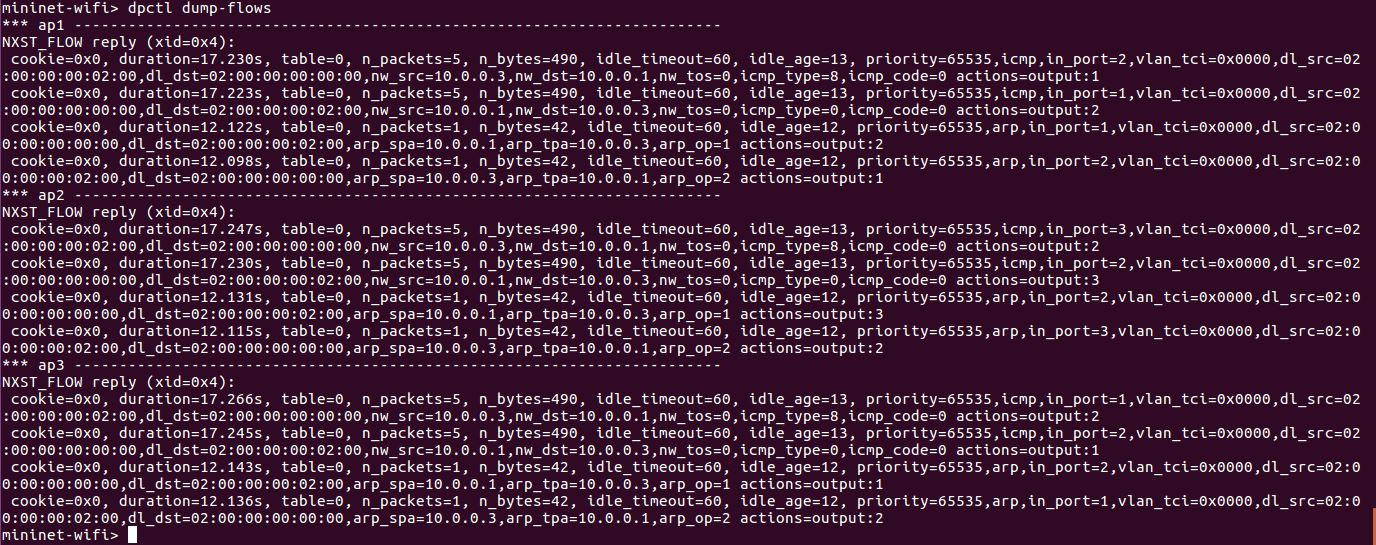
\includegraphics[width=0.9\linewidth]{./img/test/18.JPG}
    \caption{Flow tables de los distintos puntos de acceso.}
  \label{fig:yo}
\end{figure}
\newpage
Si este proceso lo hacemos lo suficientemente rápido nos daremos cuenta que al mover Sta1 el ping no funciona. Esto se debe a que las entradas de la tabla de Flows siguen configuradas para llevar un paquete desde ap3 hasta ap2, pero no a ap1. Si pasa el tiempo suficiente estas entradas serán desechadas o bien, podemos quitarlas nosotros para que se creen unas entradas en las tablas de Flows nuevas y que así se pueda alcanzar Sta1 desde su nueva posición.
\begin{itemize}
    \item \textbf{dpctl del-flows}
\end{itemize}
Llegados a este punto, ya habríamos acabado el test 2, por lo que solo nos quedaría salir y limpiar Mininet-Wifi. Como ya se explicó:

\begin{itemize}
    \item (Desde la CLI de Mininet-Wifi) exit
    \item  sudo mn -c
\end{itemize}
\newpage
\section{Test 3: Python API y scripts}

Mininet proporciona una API de Python para que los usuarios puedan crear secuencias de comandos de Python simples que configurarán 
topologías personalizadas en Mininet-WiFi. Mininet-WiFi extiende esta API para soportar un entorno inalámbrico a la ya existente API de Mininet para Python.\newline
\newline
\begin{figure}[!htb]
  \centering
    
\includegraphics[width=0.8\linewidth]{./img/test/mininet-wifi-logo.png}
\end{figure}

Cuando se usa el comando normal Mininet \textbf{mn} con la opción –-wifi para crear Mininet-WiFi, no se tiene acceso a la mayoría de las funciones ampliadas que se proporcionan en Mininet-WiFi para crear topologías. Para acceder a las funciones que le permiten emular el comportamiento de los nodos en una LAN inalámbrica, se debe
usar las extensiones de Mininet-Wifi para la API de Mininet de Python.\newline
\newline
Las grandes diferencias que tiene la nueva API de Mininet-Wifi respecto a la anterior de Mininet, es que han añadido nuevos métodos al objeto de la topología, llamados \textit{addStation} y \textit{addAccessPoint}. Además han añadido código y han modificado gran parte de él para añadir el factor wireless a los enlaces, en el método \textit{addLink}. La guía nos aconseja empezando a mirar los ejemplos de scripts ya hechos en Python.\newline

\subsection{Métodos básicos API Mininet-Wifi}
\newline
A continuación, se va a exponer los métodos más básicos para trabajar con Mininet-Wifi. En los escenarios anteriores al ser escenarios por defecto se pudo apreciar que al no suministrar valores a los parámetros de los elementos de la red, se aplicaron los valores por defecto. Ahora desde los scripts creados se podrá especificar con exactitud los valores que queremos. 

% Para los scripts 
%\begin{minted}[xleftmargin=5pt,linenos,fontsize=\small]{python}
\begin{minted}[]{python}
#De esta manera añadiríamos una estación Wifi por defecto

net.addStation( 'sta1' )


#Con esta sentencia añadiriamos un nuevo punto de acceso,
# pero a diferencia de los punto de acceso usados, 
# este no tendrá un SSID por defecto apX-ssid, si no, el suministrado.

net.addAccessPoint( 'ap1', ssid='new_ssid' )


#Para añadir un enlace Wireless entre ambos se hace con la siguiente
# sentencia, pero el enlace tendrá los valores por defecto.

net.addLink( ap1, sta1 )

\end{minted}

Para crear escenarios más complicados y complejos se puede explotar todos los posibles parámetros que recogen estos métodos. Entre los cuales, se puede indica, MAC, IP, localización (x,y,z), radio de alcance, y mucho más. Por ejemplo, el siguiente código define un punto de acceso y una estación, y crea una asociación (una conexión inalámbrica) entre los dos nodos y aplica algunos parámetros de control de tráfico a la conexión a de radio realista, agregando restricciones de ancho de banda, una tasa de error de bit y un
retardo de propagación.

\begin{minted}[]{python}

# Añadimos una estación Wifi con un método de encriptado,
# MAC, Ip, posición, contraseña y nombre.

net.addStation( 'sta1', passwd='123456789a', encrypt='wpa2',
 mac='00:00:00:00:00:02', ip='10.0.0.2/8', position='50,30,0' )
 
# Añadimos un punto de acceso indicándole, método de encriptado,
# MAC, SSID, canal, modo de wifi (Entiendo que se refieren a que tipo de estándar IEEE 
# de Wifi), posición, radio de cobertura.

net.addAccessPoint( 'ap1', passwd='123456789a', encrypt='wpa2', ssid=
 'ap1-ssid', mode= 'g', channel= '1', position='30,30,0', range=30 )

\end{minted}

Para activar la asociación de control en una red estática se debe usar el método que nos proporciona la api de Python de Mininet-Wifi que automáticamente elige el punto de acceso al cual una estación wifi debe ser conectado(Basado en la distancia entre estaciones Wifi y puntos de acceso). Por ejemplo podemos utilizar este criterio de elección \textbf{ssf} (Strongest signal first) para decidir desde una estación wifi a que punto de acceso debe ser conectada.

\begin{minted}[]{python}
net.setAssociationCtrl( 'ssf' )
\end{minted}

\subsection{Métodos básicos API Mininet }

La API de Python de Mininet sigue siendo compatible en la API de Mininet-Wifi. Añade switches host y controladores.\newline
\newline

\begin{itemize}
    \item Añadir un \textbf{Host}, la diferencia entre los host usados en Mininet-Wifi y los host convencionales de Mininet es que unos tienen una interfaz virtual de Ethernet y los de Mininet-Wifi tienen una interfaz virtual wireless.
    \begin{center}
        \textbf{net.addHost( 'h1' )}
    \end{center}
    \item Añadir un \textbf{Switch}, hay que tener en cuenta que los puntos de accesos usados en Mininet-Wifi operan como switches pero con interfaz virtual wireless. 
    \begin{center}
        \textbf{net.addSwitch( 's1' )}
    \end{center}
    \item Añadir un \textbf{Link}, de tipo Ethernet entre dos nodos de la red. Por lo visto según la gui al enlazar dos Puntos de acceso por defecto se emplea en enlace de Ethernet.
    \begin{center}
        \textbf{net.addLink( s1, h1 )}
    \end{center}
    \item  Añadir un controlador.
        \begin{center}
        \textbf{net.addController( 'c0' )}
    \end{center}
\end{itemize}
Podemos contemplar que con esta combinación de la API anterior de Mininet más los añadidos con Mininet-Wifi nos da la posibilidad de construir una topología que incluya host, switches, estaciones wifi, puntos de acceso y múltiples controladores. 
\newpage
\subsection{Ejemplo script Mininet-Wifi}
\begin{minted}[xleftmargin=5pt,linenos,fontsize=\small]{python}
#!/usr/bin/python

from mininet.node import Controller
from mininet.log import setLogLevel, info
from mn_wifi.node import OVSKernelAP
from mn_wifi.cli import CLI_wifi
from mn_wifi.net import Mininet_wifi


def topology():
   
    net = Mininet_wifi(controller=Controller, accessPoint=OVSKernelAP)

    info("*** Creamos los nodos de la topologia\n")
    sta1 = net.addStation('sta1', mac='00:00:00:00:00:02', ip='10.0.0.2/8',
                          range=20, position='10,20,0')
    sta2 = net.addStation('sta2', mac='00:00:00:00:00:03', ip='10.0.0.3/8',
                          range=20, position='50,20,0')
    ap1 = net.addAccessPoint('ap1', ssid='ssid-ap1', mode='g', channel='1',
                             position='15,30,0', range=30)
    ap2 = net.addAccessPoint('ap2', ssid='ssid-ap2', mode='g', channel='6',
                             position='55,30,0', range=30)
    c1 = net.addController('c1', controller=Controller)

    #Config nodos   
    info("*** Configuramos los nodos de la topologia\n")
    net.configureWifiNodes()
    net.setAssociationCtrl('ssf')

    #Matplotlib dibujo 
    net.plotGraph(max_x=100, max_y=100)

    #Enlaces 
    info("*** Creamos los links\n")
    net.addLink(ap1, ap2)
    net.addLink(ap1, sta1)
    net.addLink(ap2, sta2)

    info("*** Arrancar la red\n")
    net.build()
    c1.start()
    ap1.start([c1])
    ap2.start([c1])

    info("*** MininetWifi CLI ...\n")
    CLI_wifi(net)

    info("*** Parar la red\n")
    net.stop()


if __name__ == '__main__':
    setLogLevel('info')
    topology()

\end{minted}
En este ejemplo hemos tenido una dificultad, y es el método de la topología que establece el criterio de asociación entre estaciones Wifi y puntos de acceso. En la documentación lo expone según \textbf{associationControl()} y en la API se llama \textbf{setAssociationCtrl()} . 
\newpage
Se ha abierto un Issue indicándole a los creadores y a los desarrolladores que mantienen el proyecto si pueden cambiarlo o poner una nota para que la gente que inicia leyendo la documentación no tenga dificultades añadidas. \newline
\newline
\begin{center}
\url{https://github.com/intrig-unicamp/mininet-wifi/issues/226}
\end{center}

\begin{figure}[!htb]
  \centering
    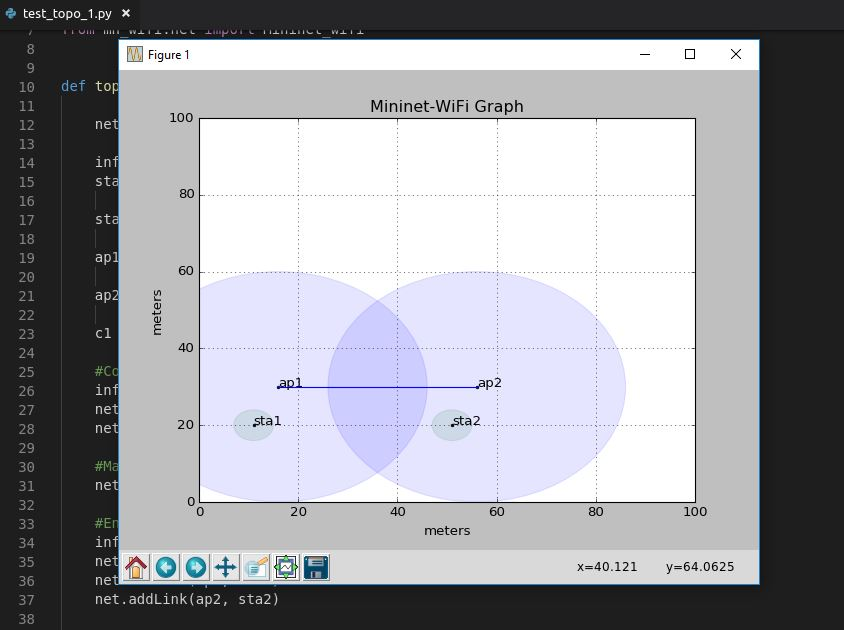
\includegraphics[width=0.9\linewidth]{./img/test/19.JPG}
    \caption{Resultado de ejecución del ejemplo.}
  \label{fig:yo}
\end{figure}
El script lo hemos ejecutado desde la terminal haciendo uso del interprete de comandos. Lo hemos invocado según el siguiente comando:
\begin{itemize}
    \item sudo python test\_topo\_1.py
\end{itemize}
También se podría haber ejecutado directamente siempre y cuando el Path del interprete estuviera bien puesto. Una vez ejecutado el script, tendremos una topología cargada en Mininet-Wifi de dos puntos de acceso y dos estaciones Wifi emparejadas a cada uno de estos puntos de acceso. \newline
\newline
Como hemos indicado en el script que queríamos que cargase la CLI de Mininet-Wifi y que dibujara la topología, al completar la ejecución del script entrará en la CLI de Mininet-Wifi y con ayuda de matplotlib graficará la topología.
Una vez dentro de la CLI de Mininet-Wifi podremos consultar los parámetros tales como la posición de un nodo de la topología. Esto lo podemos hacer haciendo del comando \textbf{py} que incorpora la CLI. Además, por lo que hemos podido ver, la CLI soporta código de python directamente haciendo uso del comando \textbf{py}. Esto será muy util para consultar información o para hacer breves cambios en la red cuando el escenario ya está corriendo.
\newpage
\begin{figure}[!htb]
  \centering
    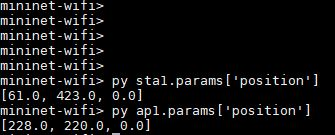
\includegraphics[width=0.6\linewidth]{./img/test/20.JPG}
    \caption{Consultar parámetros desde la CLI.}
  \label{fig:yo}
\end{figure}

\subsection{Cambiando la red durante el tiempo de ejecución}

Mininet-WiFi proporciona funciones de Python que se pueden usar durante el tiempo de ejecución para realizar cambios en el nodo en lo relativo a posiciones y asociaciones. Estas funciones son útiles cuando tenemos una configuración estática y queremos hacer cambios puntuales.\newline
\newline
Para cambiar el punto de acceso al que está asociada una estación wifi (siempre que la estación Wifi esté en el rango del punto de acceso a cambiar):
\begin{minted}[]{python}
mininet-wifi> py sta1.setAssociation('sta1-wlan0', ap1)
\end{minted}
Para mover una estación Wifi o un punto de acceso dado unas coordenadas en el espacio. Formato (X,Y,Z).
\begin{minted}[]{python}
mininet-wifi> py sta1.setPosition('40,20,40')
\end{minted}
También podemos modificar a tiempo real el rango de un punto de acceso.
\begin{minted}[]{python}
mininet-wifi> py sta1.setRange(100)
\end{minted}
Las modificaciones que hagamos vía CLI repercutirán directamente en el funcionamiento de la red. Un cambio de posición de asociación puede ser clave en el desempeño en la operativa de funcionamiento de la red.
\newline
\newline
Llegados a este punto, ya habríamos acabado el test 3, por lo que solo nos quedaría salir y limpiar Mininet-Wifi. Como ya se explicó:

\begin{itemize}
    \item (Desde la CLI de Mininet-Wifi) exit
    \item  sudo mn -c
\end{itemize}
\newpage
\section{Test 4}
En este test se va a explorar una de las funcionalidades más importantes de Mininet-Wifi, la movilidad. Mininet-Wifi proporciona nuevos métodos en su API de Python, como \textit{startMobility} y \textit{Mobility}, con lo que podemos especificar una amplia variedad de escenarios de LAN inalámbrica mediante el control
movimiento de la estación Wifi.

\subsection{Python API y métodos de movilidad}
La API de Python de Mininet-WiFi agrega nuevos métodos que permiten al usuario crear estaciones que se mueven alrededor en el espacio virtual cuando se ejecuta un escenario de emulación.\newline
\newline
Para mover una estación en línea recta, use los métodos \textbf{net.startMobility}, \textbf{net.mobility} y \textbf{net.stopMobility}. Por ejemplo, para mover una estación Wifi de una posición a
otra durante un período de 60 segundos.
\begin{minted}[]{python}
net.startMobility( time=0 )
net.mobility( sta1, 'start', time=1, position='10,20,0' )
net.mobility( sta1, 'stop', time=59, position='30,50,0' )
net.stopMobility( time=60 )
\end{minted}
Mininet-WiFi también puede mover estaciones wifi de forma automática según los modelos de movilidad predefinidos. Los modelos de movilidad disponibles son:
\begin{itemize}
    \item RandomWalk
    \item TruncatedLevyWalk
    \item RandomDirection
    \item RandomWayPoint
    \item GaussMarkov
    \item ReferencePoint
    \item TimeVariantCommunity
\end{itemize}
Por ejemplo, para mover una estación en un área de 60 metros por 60
metros, con una velocidad mínima de 0.1 metros por segundo y una velocidad máxima de 0.2 metros por segundo.
\begin{minted}[]{python}
net.setMobilityModel(time=0, model='RandomDirection', max_x=60, 
 max_y=60, min_v=0.1, max_v=0.2)
\end{minted}
Mininet-WiFi conectará y desconectará automáticamente las estaciones desde y hacia los puntos de acceso en función de la intensidad de señal calculada o el nivel de carga en ese punto de acceso. 
\newline
\newline
Para utilizar un método de control de asociación, necesita agregue el parámetro AC en net.setMobilityModel(). Por ejemplo, para cambiar los puntos de acceso basados en
los criterios de "menos cargado primero":
\begin{minted}[]{python}
net.setMobilityModel(time=0, model='RandomWayPoint', max_x=140,
  max_y=140, min_v=0.7, max_v=0.9, AC='llf')
\end{minted}

Por lo que tendríamos dos criterios de asociación a un punto de acceso.

\begin{itemize}
    \item llf  (Least-Loaded-First)
    \item ssf  (Strongest-Signal-First)
\end{itemize}
\newpage
\subsection{Ejemplo script movilidad}

\begin{minted}[xleftmargin=5pt,linenos,fontsize=\small]{python}
#!/usr/bin/python



from mininet.node import Controller
from mininet.log import setLogLevel, info
from mn_wifi.net import Mininet_wifi
from mn_wifi.node import OVSKernelAP
from mn_wifi.cli import CLI_wifi



def topo():


	net = Mininet_wifi(controller= Controller, accessPoint = OVSKernelAP)
	
	info("*** Creando nodos\n")
	h1 = net.addHost( 'h1', mac='00:00:00:00:00:01',ip='10.0.0.1/8') 
	
	sta1 = net.addStation( 'sta1', mac='00:00:00:00:00:02',ip='10.0.0.2/8', range ='20')
	
	ap1 = net.addAccessPoint('ap1', ssid = 'ap1-ssid', mode='g', channel= '1', 
	position='30,50,0', range='30')
	
	ap2 = net.addAccessPoint('ap2', ssid = 'ap2-ssid', mode='g', channel= '1', 
	position='90,50,0', range='30')
	
	ap3 = net.addAccessPoint('ap3', ssid = 'ap3-ssid', mode='g', channel= '1', 
	position='150,50,0', range='30')
	
	c1 = net.addController('c1' , controller = Controller)

	info("*** Configurando nodos\n")
	net.configureWifiNodes()


	info("*** Creando links\n")
	net.addLink(ap1, h1)
	net.addLink(ap1, ap2)
	net.addLink(ap2,ap3)

	info("*** Dibujando Topo con matplotlib\n")
	net.plotGraph(max_x=200, max_y = 200)

	info("*** Configurando Movilidad (sta1)\n")
	net.startMobility(time = 0, AC='ssf')
	net.mobility(sta1, 'start', time = 20, position='1,50,0')
	net.mobility(sta1, 'stop', time = 79, position='159,50,0')
	net.stopMobility(time=200)

	info("*** Network UP!\n")
	net.build()
	c1.start()
	ap1.start([c1])	
	ap2.start([c1])	
	ap3.start([c1])	



	info("*** Cargamos Mininet-Wifi CLI\n")
	CLI_wifi(net)

	info("*** Parando network\n")
	net.stop()


if __name__ == '__main__':
	setLogLevel('info')
	topo()

\end{minted}

Nos hemos dado cuenta que para que complete su recorrido desde x=1 a x=159 debemos darle más tiempo de movilidad por lo que hemos aumentado el periodo de movilidad hasta 200 segundos, ya que con los 79 segundos apenas llegaba a la mitad del recorrido. \newline
\newline
\begin{center}
    \url{https://github.com/davidcawork/testMininet-Wifi/blob/master/doc/Topologies_img/test_movilidad_1.gif}
\end{center}

Podemos hacer uso del comando \textbf{py} de la CLI de Mininet-Wifi para obtener información relativa a que punto de acceso estamos en rango, esto es muy útil para ver en que momento la estación Wifi está en un conflicto y debe aplicar el criterio de selección para decidir a que punto de acceso conectarse.

\begin{minted}[]{python}
mininet-wifi> py sta1.params['apsInRange']
[<OVSAP ap1: lo:127.0.0.1,ap1-wlan1:None,ap1-eth2:None,ap1-eth3:None pid=28721> ]
mininet-wifi> py sta1.params['apsInRange']
[<OVSAP ap2: lo:127.0.0.1,ap2-wlan1:None,ap2-eth2:None,ap2-eth3:None pid=28727> ]

# Handover entre dos células de Ap1 a Ap2 

\end{minted}

\subsection{Prueba con la herramienta Iperf}
En esta prueba se va a utilizar la topología expuesta en el punto anterior(test\_movilidad\_1.py). La operativa va a ser de generar tráfico TCP  entre una estación Wifi y un host estático con Iperf. Nuestro servidor será la estación wifi dotada de movilidad, que irá recorriendo los tres puntos de acceso ap1, ap2  y ap3. \newline
\newline
El objetivo de la prueba es ver en el momento del handover entre dos puntos de acceso, como el tráfico deja de fluctuar entre servidor y cliente. Esto se debe a que las reglas instauradas por el controlador en el ap1 dejan de ser útiles ya que este se encuentra en el dominio del ap2 por lo que el trafico deja de fluctuar. Para resolverlo podemos eliminar las reglas instauradas con \textbf{dpctl del-flows}. Pasos a seguir:
\begin{itemize}
    \item sudo python test\_movilidad\_1.py
    \item xterm sta1
    \item xterm h1
    \item (En la consola de sta1) iperf --server
    \item (En la consola de h1) iperf --client 10.0.0.2 --time 60 --interval 2
    \item Observar como deja de fluctuar el tráfico tras producirse el handover.
    \item dpctl del-flows
    \item Se recupera el tráfico.
\end{itemize}
\newpage
\begin{figure}[!htb]
  \centering
    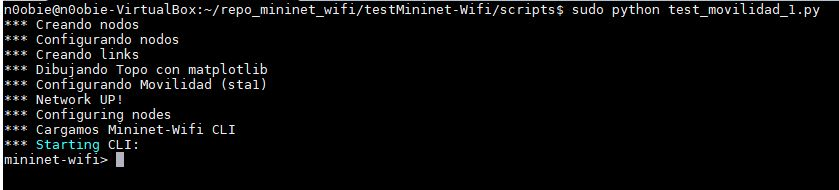
\includegraphics[width=0.8\linewidth]{./img/test/21.JPG}
    \caption{Levantamos la topología.}
  \label{fig:yo}
\end{figure}
\begin{figure}[!htb]
  \centering
    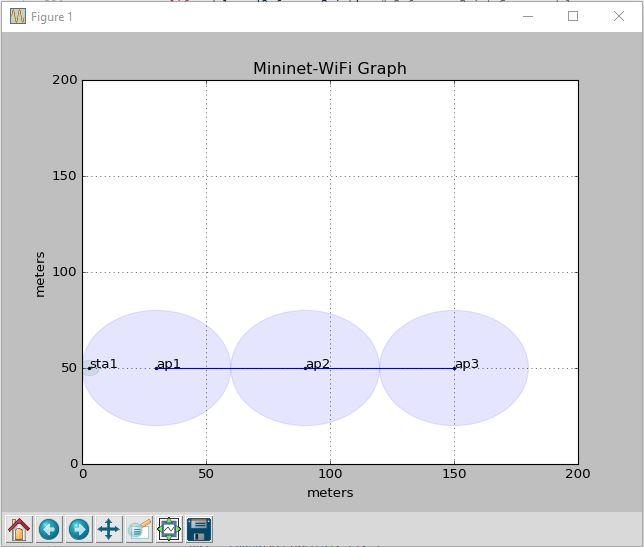
\includegraphics[width=0.6\linewidth]{./img/test/22.JPG}
    \caption{Topología Inicial.}
  \label{fig:yo}
\end{figure}
\newpage
\begin{figure}[!htb]
  \centering
    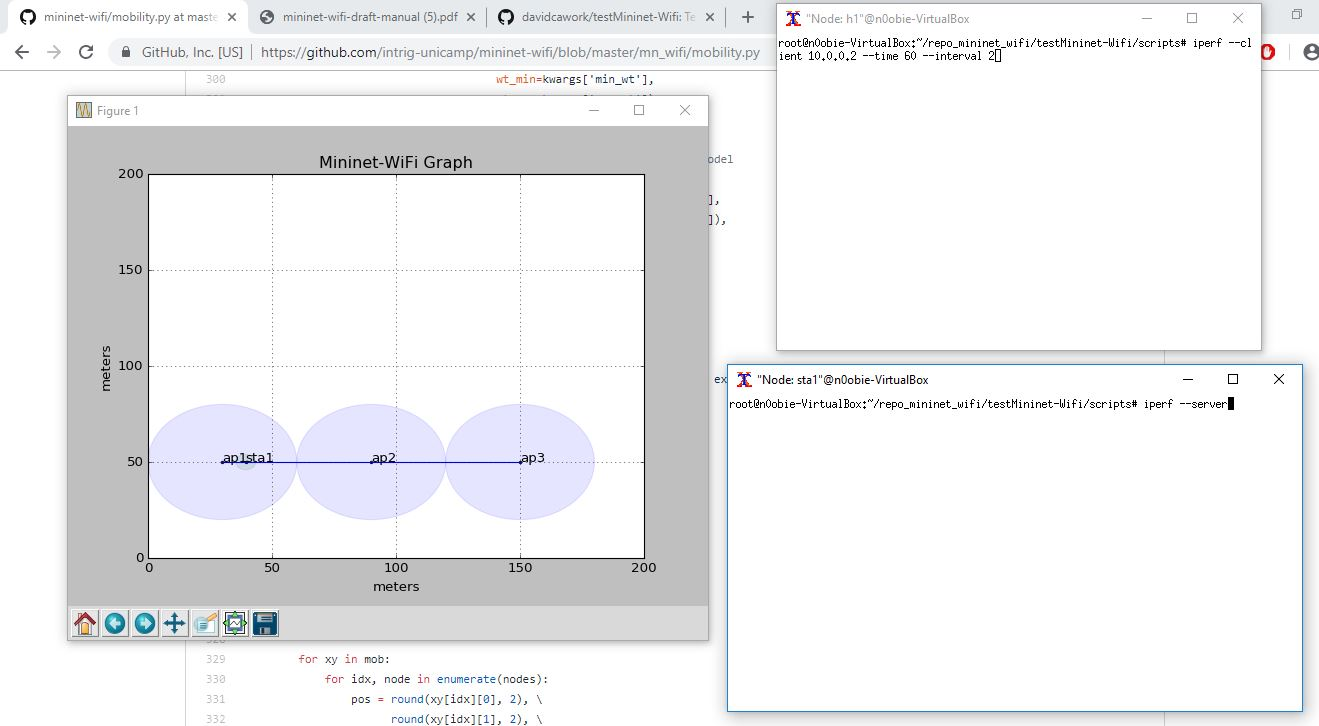
\includegraphics[width=\linewidth]{./img/test/23.JPG}
    \caption{Lanzamos las consolas en Sta1 y h1.}
  \label{fig:yo}
\end{figure}
\begin{figure}[!htb]
  \centering
    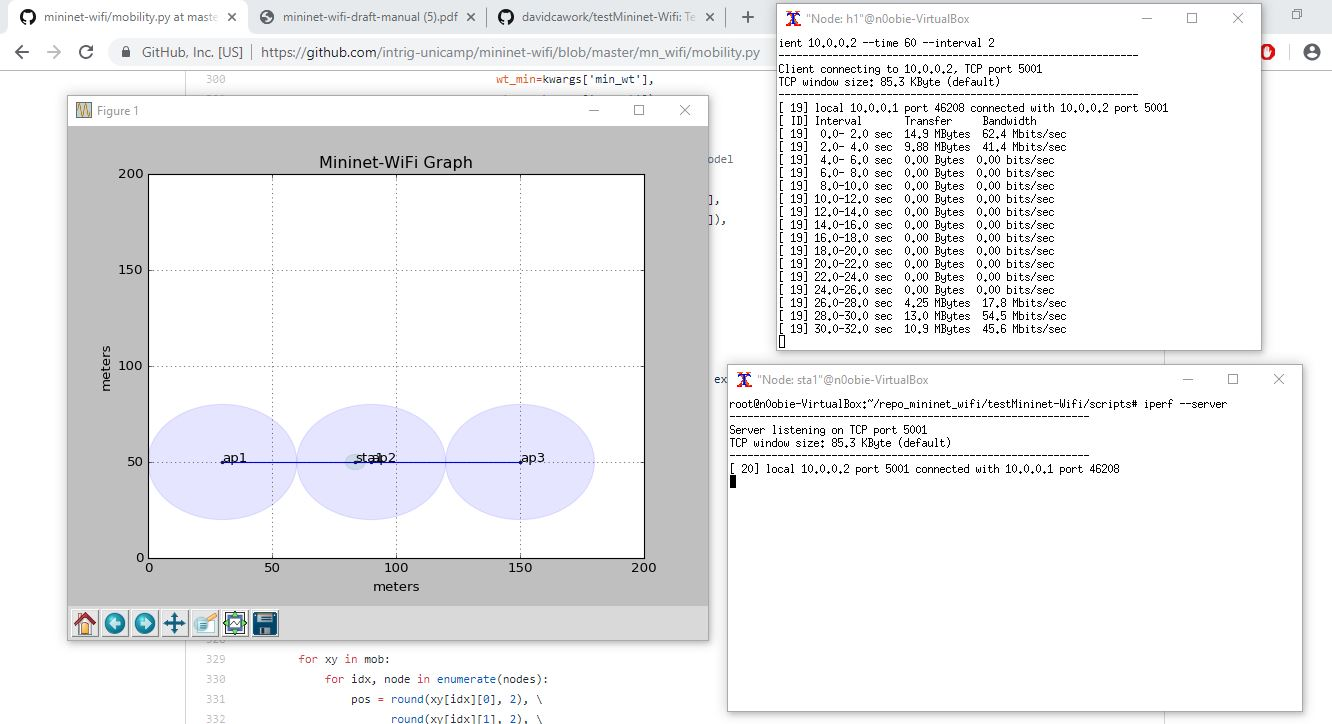
\includegraphics[width=\linewidth]{./img/test/24.JPG}
    \caption{Creamos tráfico entre Sta1 y h1.}
  \label{fig:yo}
\end{figure}
\newpage
\begin{figure}[!htb]
  \centering
    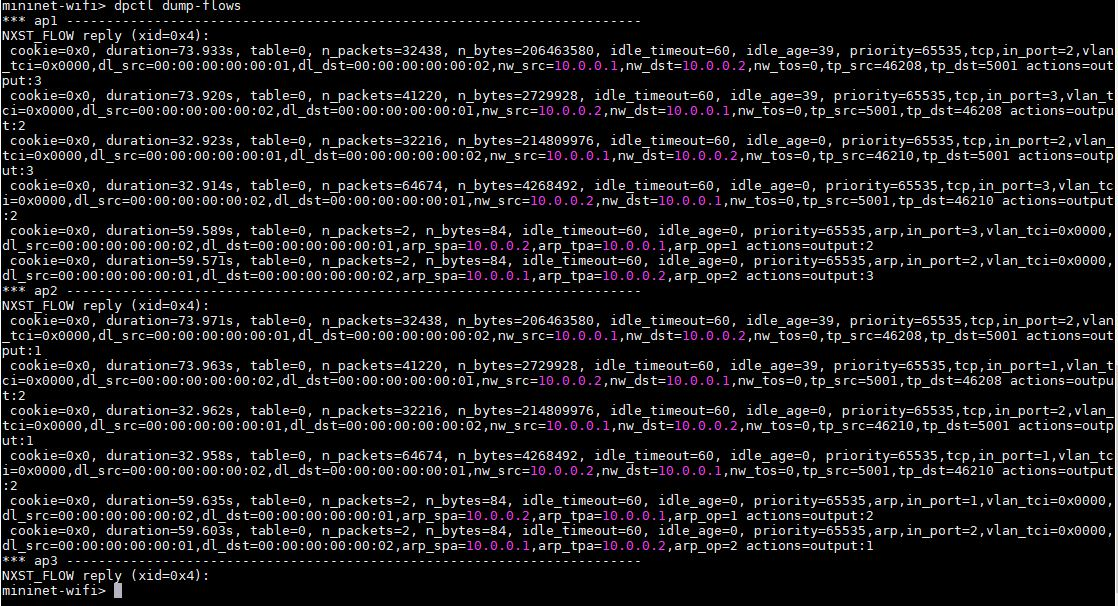
\includegraphics[width=\linewidth]{./img/test/25.JPG}
    \caption{Tablas antes del Handover.}
  \label{fig:yo}
\end{figure}
\begin{figure}[!htb]
  \centering
    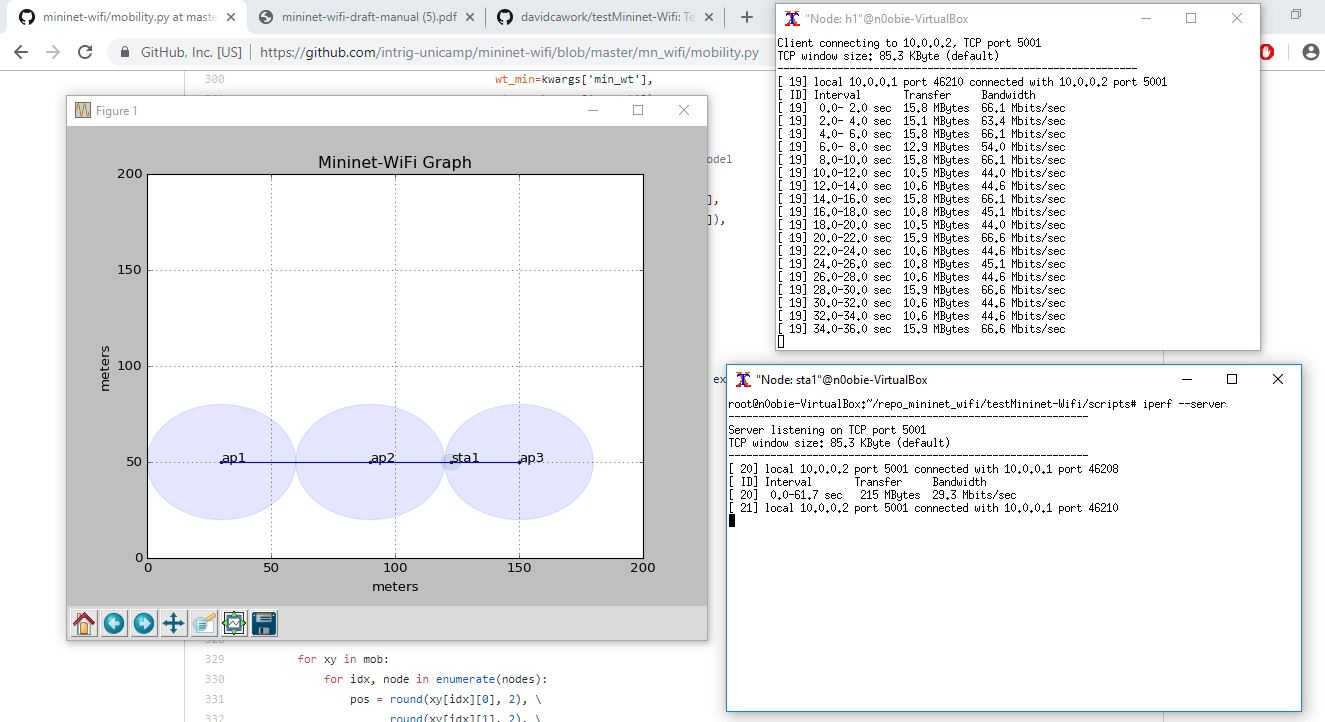
\includegraphics[width=\linewidth]{./img/test/26.JPG}
    \caption{Handover realizado el tráfico se detiene.}
  \label{fig:yo}
\end{figure}
\newpage
\begin{figure}[!htb]
  \centering
    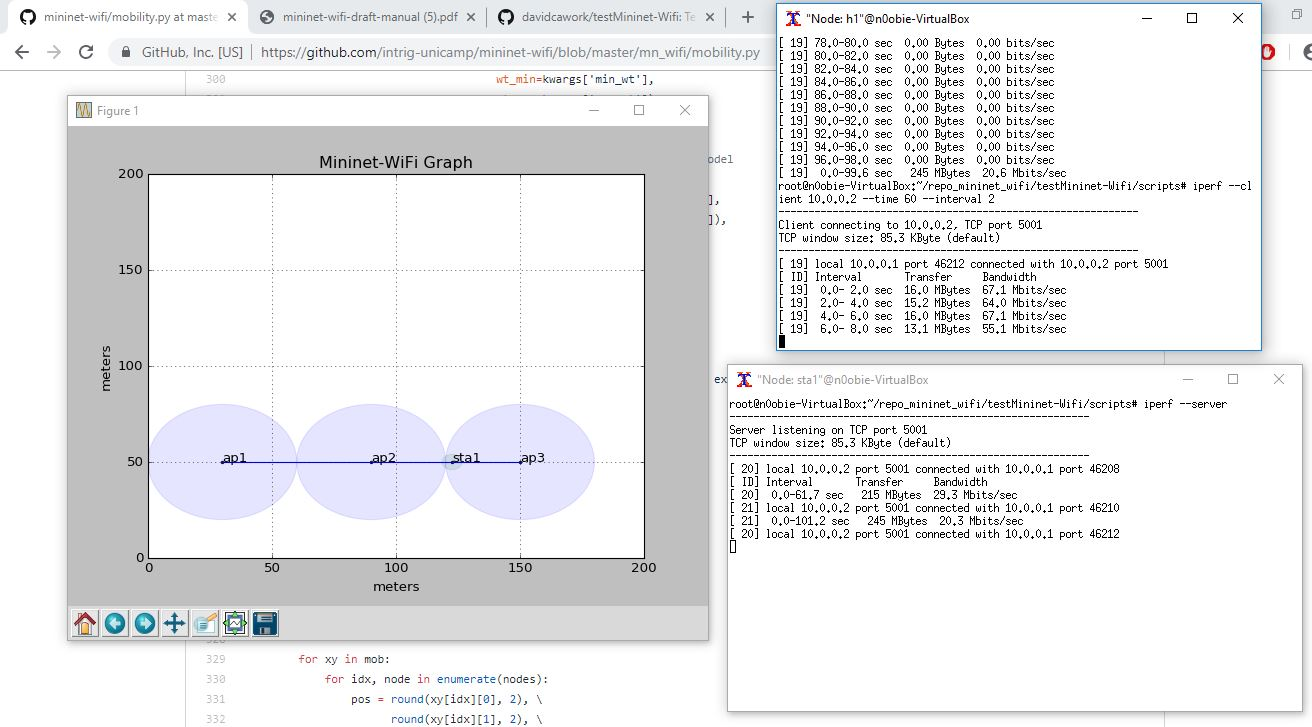
\includegraphics[width=\linewidth]{./img/test/27.JPG}
    \caption{Borramos las tablas, el tráfico se recupera pasados unos segundos.}
  \label{fig:yo}
\end{figure}
Llegados a este punto, ya habríamos acabado el test 4, por lo que solo nos quedaría salir y limpiar Mininet-Wifi. Como ya se explicó:
\begin{itemize}
    \item (Desde la CLI de Mininet-Wifi) exit
    \item  sudo mn -c
\end{itemize}